\section{Informationstheorie }
\subsection{Informationsgehalt, Binary Unit, Entropie, Informationsrate}
Mathematisch gesehen kann man sagen, je \textbf{unwahrscheinlicher} das \textbf{Eintreten} eines \textbf{spezifischen
Ereignisses} ist, desto \textbf{gr�sser} ist dessen \textbf{Informationsgehalt}. \\

\begin{minipage}[c]{13cm}
	$$ I(x_i) = \log_{base} \frac{1}{P(x_i)} = - \log_{base} P(x_i) \qquad \qquad  R = r H (X)$$
	$$ H(X) = E[I(x_i)] = \sum\limits_{i=1}^m P(x_i) I(x_i) = - \sum\limits_{i=1}^m P(x_i)
	\log_2{P(x_i)} \qquad 0 \leq H(x) \leq \log_2(m)$$
	$$ H(X|Y)=- \sum\limits_{j=1}^{n} \sum\limits_{i=1}^{m} P(x_i,y_j)
	log_2(P(x_i|y_j))$$
	$$ H(X,Y)=- \sum\limits_{j=1}^{n} \sum\limits_{i=1}^{m}
	P(x_i,y_j)log_2(P(x_i,y_j)) =H(X)+HY|Y)=H(Y) + H(X|Y)$$
	$$I(X;Y)=I(Y;X)=H(X)+H(Y)-H(X,Y)=H(X)-H(X|Y)$$
	\textbf{Bin�re Entropie:}
	$$u(P(x_i))=-P(x_i) log_2(P(x_i))-(1-P(x_i) log_2(1-P(x_i)))$$
\end{minipage}
\begin{minipage}[c]{7cm}
	$I(x_i)$ Informationsgehalt, $[I(x_i)] = b$ \\\\
	$base = 2$ siehe nachfolgender Text\\\\
	$P(x_i)$ Auftretens-WSK eines Symbols \\\\
	$H(x_i)$ Entropie, $[H(x_i)] = $ b/Symbol \\\\
	$R$ Informationsrate, $[R]$ = b/s  \\\\
	$r$ Symbolrate, $[r]$ = Symbole/s 
%	$$
\end{minipage}
\vspace{0.2cm} \\
Der Informationsgehalt kann in folgenden Masseinheiten angegeben werden: \\
$$ [I(X)] = \begin{cases}
            	\text{bit (\emph{bi}nary uni\emph{t})}
            		& \text{falls } base=2. \\
            	\text{hartley oder decit}
            		& \text{falls } base=10. \\
            	\text{nat (\emph{na}tural uni\emph{t})}
            		& \text{falls } base=e
			\end{cases} $$

\textbf{Standartm�ssig} verwenden wir $base=2$, also bit oder gek�rzt \textbf{b}. Binary Unit ist
ein Mass f�r den Informationsgehalt und sollte nicht mit dem Term ``bit'' (Bin�res Zeichen) verwechselt
werden.

\subsection{DMS - Discrete Memoryless Source}
Eine Informations\textbf{quelle} ist ein Objekt welches \textbf{Ereignise}, welche zuf�llig aus einer
WSK-Dichtefunktion ausgew�hlt werden, \textbf{generiert}. \\
Eine diskrete Quelle hat einen endlichen \textbf{Satz an Symbolen}, welcher auch \textbf{Alphabet}
genannt wird. Die Elemente dieses Satzes nennt man \textbf{Symbole} oder \textbf{Zeichen}. \\
Wird ein Symbol unabh�ngig vom Vorherigen generiert, so handelt es sich um eine DMS (diskrete
ged�chtnisfreie Quelle). Eine solche wird mit folgenden Eigenschaften charakterisiert:
\begin{itemize}
  \item Liste der Symbole - Alphabet
  \item Auftretenswahrscheinlichkeiten dieser Symbole - WSK-Dichtefunktion
  \item Symbolrate
\end{itemize}


\subsection{DMC - Discrete Memoryless Channels}
\begin{minipage}{9.5cm}
	\begin{center}
		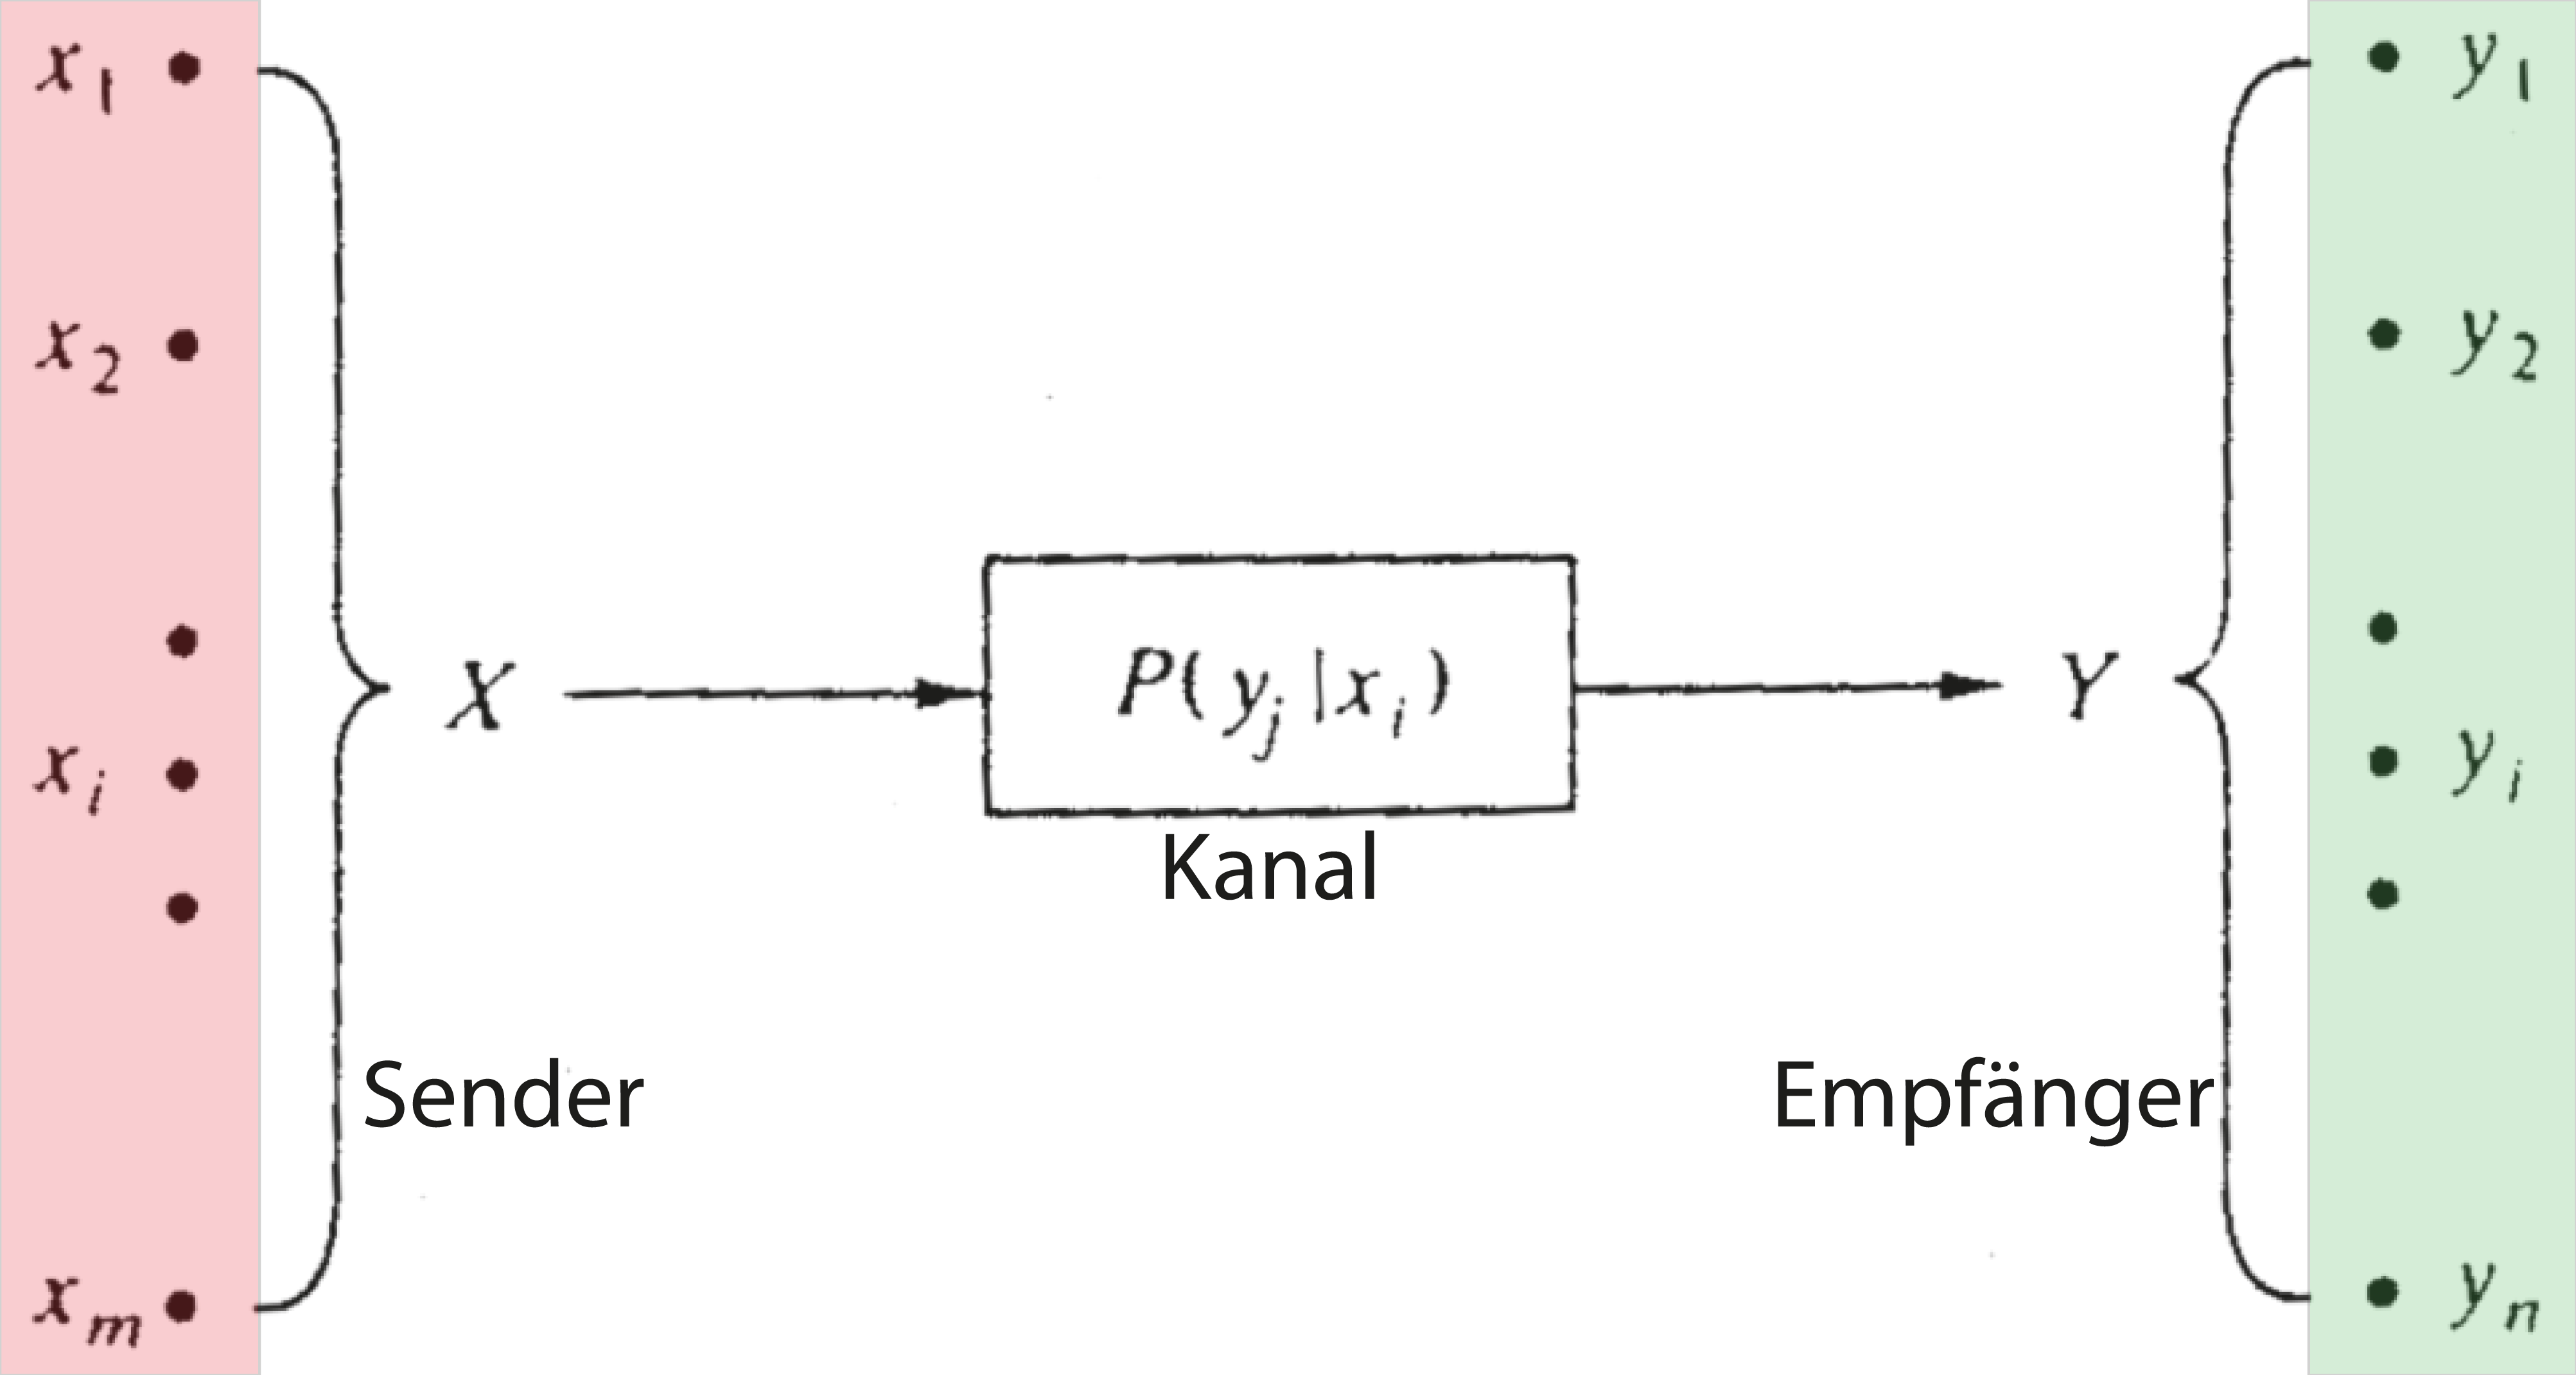
\includegraphics[width=8cm]{../NaT2/bilder/10_DMC.png}
	\end{center}
\end{minipage}
\begin{minipage}{8.5cm}
	Ein DMC (diskreter ged�chtnisfreier Kanal) ist ein statistisches Modell mit Eingang $X$ und
	Ausgang $Y$. \\ \\
	Er besitzt \textbf{$m$ Eing�nge} und \textbf{$n$ Ausg�nge}. \\ \\
	Alle Auftretenswahrscheinlichkeiten $P(x_i)$ der einzelnen Eingangs-Symbole werden als gegeben
	betrachtet. \\
	Jeder �bertragungspfad ist durch die Kanal-�bertragungs-Wahrscheinlichkeiten (channel transition
	probabilities) $P(y_j | x_i)$ definiert.
\end{minipage}

\subsubsection{Darstellung in Matritzenform}
\begin{minipage}{9cm}
	\textbf{Kanalmatrix}
	$$ [P(Y | X)] = \begin{bmatrix}
              P(y_1 | x_1) & P(y_2 | x_1) & \ldots & P(y_n | x_1) \\
              P(y_1 | x_2) & P(y_2 | x_2) & \ldots & P(y_n | x_2) \\
             \vdots & \vdots & \vdots & \vdots \\
              P(y_1 | x_m) & P(y_2 | x_m) & \ldots & P(y_n | x_m)
           \end{bmatrix}$$ \\
	$ [P(Y)] = [P(X)] \cdot [P(Y|X)]$ und $\sum\limits_{j=1}^n P(y_j | x_i) = 1 (\forall i)$
\end{minipage}
\begin{minipage}{9cm}
	\textbf{Verbundmatrix}
	$$ [P(Y,X)] = \begin{bmatrix}
              P(y_1, x_1) & P(y_2, x_1) & \ldots & P(y_n, x_1) \\
              P(y_1, x_2) & P(y_2, x_2) & \ldots & P(y_n, x_2) \\
             \vdots & \vdots & \vdots & \vdots \\
              P(y_1, x_m) & P(y_2, x_m) & \ldots & P(y_n, x_m)
           \end{bmatrix}$$
	$  [P(Y,X)] =  [P(X)]_d [P(Y|X)] $ \\
	Elemente auf der Diagonale sollten den gr�ssten Wert gegen�ber anderen Elementen auf der Zeile
	besitzen.
\end{minipage}

\subsubsection{Spezielle Kan�le}

\textbf{uniformly Dispersive} \\
\begin{minipage}{10cm}
Ein Kanal ist uniformly Dispersive, wenn ide WSK von einem Eingang zu den
Ausg�nge gleich wie bei den anderen Eing�ngen ist. z.B.:
\end{minipage}
\begin{minipage}{9cm}
	$$ [P(Y | X)] = \begin{bmatrix}
              \frac34 & \frac14 &  0 & 0 \\
              0 & \frac34 & \frac14 & 0 \\
              0 & 0 & \frac34 & \frac14 \\
              \frac14 &  0 & 0 &\frac34 \\
           \end{bmatrix}$$ \\
\end{minipage}        
           
\textbf{Verlustfreier(lossless) Kanal}\\
\begin{minipage}{14cm}
	Auf jeder Spalte der Kanalmatrix gibt es jeweils nur ein  Element $\neq 0$. \\

	$$ [P(Y | X)] = \begin{bmatrix}
              \frac34 & \frac14 & 0 & 0 & 0 \\
              0 & 0 & \frac13 & \frac23 & 0 \\
              0 & 0 & 0 & 0 & 1
           \end{bmatrix}$$ 
\end{minipage}
\begin{minipage}{4cm}
\begin{center}
	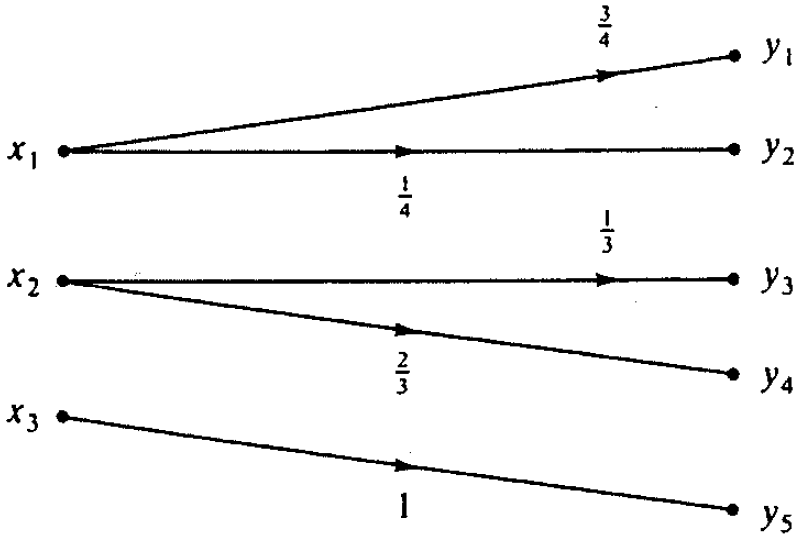
\includegraphics[height=3cm]{../NaT2/bilder/10_channels_lossless.png}
\end{center}
\end{minipage}

\textbf{Deterministischer (deterministic) Kanal} \\
\begin{minipage}{14cm}
	Auf jeder Zeile der Kanalmatrix gibt es jeweils nur ein  Element $\neq 0$, welches $1$ sein
	muss.

	$$ [P(Y | X)] = \begin{bmatrix}
           		1 & 0 & 0 \\
           		1 & 0 & 0 \\
           		0 & 1 & 0 \\
           		0 & 1 & 0 \\
           		0 & 0 & 1
           \end{bmatrix}$$
\end{minipage}
\begin{minipage}{4cm}
\begin{center}
	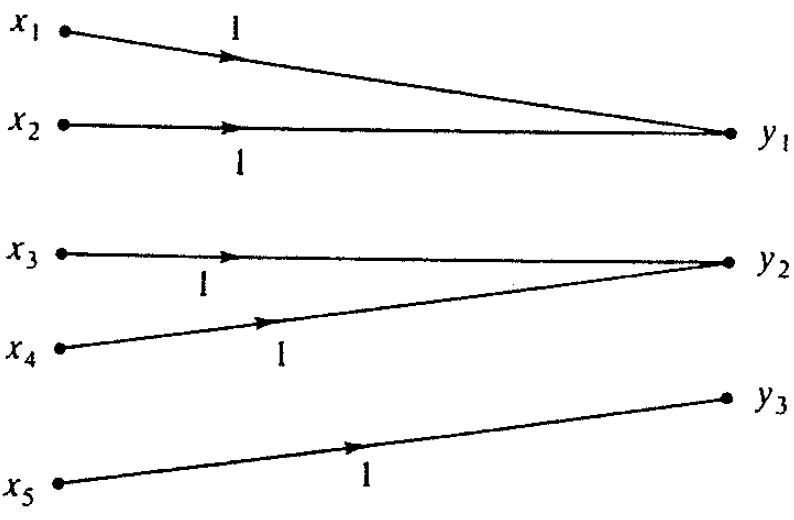
\includegraphics[height=3cm]{../NaT2/bilder/10_channels_deterministic.png}
\end{center}
\end{minipage}

\textbf{Rauschfreier (noiseless) Kanal} \\
\begin{minipage}{14cm}
	Die Kanalmatrix entspricht der Einheitsmatrix.

	$$ [P(Y | X)] = \begin{bmatrix}
           		1 & 0 & \ldots & 0\\
           		0 & 1 & \ldots & 0\\
           		\vdots & \vdots & \vdots & \vdots \\
           		0 & 0 & \ldots & 1\\
           \end{bmatrix} = I$$ \\
\end{minipage}
\begin{minipage}{4cm}
\begin{center}
	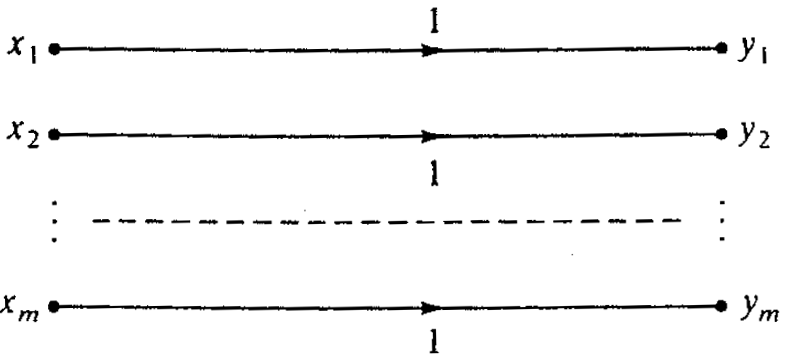
\includegraphics[width=4.5cm]{../NaT2/bilder/10_channels_noiseless.png}
\end{center}
\end{minipage}

\textbf{BSC- Bin�rer Symmetrischer (binary symmetrical) Kanal} \\
\begin{minipage}{14cm}

	$$ [P(Y | X)] = \begin{bmatrix}
           		1-p & p \\
           		p & 1-p
           \end{bmatrix} $$
\end{minipage}
\begin{minipage}{4cm}
\begin{center}
	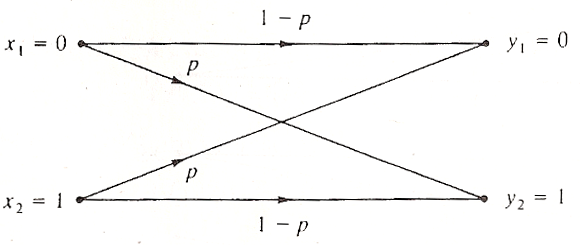
\includegraphics[width=4.5cm]{../NaT2/bilder/10_channels_binarysymmetrical.png}
\end{center}
\end{minipage}


\textbf{BEC - Bin�rer Ausl�schungs (binary erasure) Kanal} \\
\begin{minipage}{14cm}

	$$ P_{Y | X}(0|1) =  P_{Y | X}(1|0) = 0 $$
	$$ P_{Y | X}(0|0) =  P_{Y | X}(1|1) = 1-\delta $$
	$$ P_{Y | X}(\delta|0) =  P_{Y | X}(\delta|1) = \delta $$
\end{minipage}
\begin{minipage}{4cm}
\begin{center}
	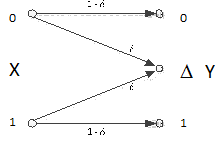
\includegraphics[width=4.5cm]{./bilder/10_channels_binaryErasure.png}
\end{center}
\end{minipage}

\textbf{Uniformly dispersive Canal} \\
Wenn die Wahrscheinlich (in einem Vektor angeorgnet und sortiert) gleich sind.
\\
z.B. $$
[\frac{1}{2},\frac{1}{4},\frac{1}{4}]=[\frac{1}{2},\frac{1}{4},\frac{1}{4}]\neq
[\frac{1}{2},\frac{1}{2}]$$


\subsection{Kanalkapazit�t}
\begin{minipage}[c]{8cm}
	$$ C_s = \max\limits_{\{ P(x_i) \}}{I (X; Y)} 
	 = \max\limits_{\{ P(x_i)\}}{H(X)- H(X|Y)} $$
	$$ = \max\limits_{\{ P(x_i)\}}{H(Y)- H(Y|X)} $$ 
	$$ C = r C_s $$
\end{minipage}
\begin{minipage}[c]{10cm}
	$C_s$ Kanalkapazit�t pro Symbol, $[C_s]$ = b/Symbol \\
	$C$ Kanalkapazit�t pro Sekunde, $[C]$ = b/s \\
	$r$ Symbolrate, $[r]$ = Symbol/s
%	$$
\end{minipage}\\
Wenn Informationsrate  $R < C \Rightarrow \epsilon = Fehlerrate = 0$  ist
m�glich


\subsection{AWGN-Channel}
AWGN = Additiv White Gausian Noise. $y(t)=x(t)+w(t)$ $w(t)$: white noise with
spectral density $\frac{N_0}2$

\subsubsection{Kanalkapazit�tien spezieller Kan�le}

	\renewcommand{\arraystretch}{2}
	\begin{tabular}{| p{3.5cm} | p{7.5cm} | p{6.5cm} |}
		\hline
    		\textbf{Verlustfrei}
    			& $ I(X; Y) = H(X) $
    			& $ C_s = \max\limits_{\{ P(x_i) \}}{H (X)} = \log_2 m $ \\
		\hline
    		\textbf{Deterministisch}
    			& $ I(X; Y) = H(Y) $
    			& $ C_s = \max\limits_{\{ P(x_i) \}}{H (Y)} = \log_2 n $ \\
		\hline
    		\textbf{Rauschfrei}
    			& $ I(X; Y) = H(Y) = H(X)$
    			& $ C_s = \log_2 n = \log_2 m$ \\
		\hline
    		\textbf{Bin�r Symmetrisch}
    			& $ I(X; Y) = H(Y) + p \log_2 p + (1-p) \log_2 (1-p)$
    			& $ C_s = 1 + p \log_2 p + (1-p) \log_2 (1-p)$ \\
		\hline
    		\textbf{Bin�r Symmetrisch}
    			& & $ C_s = 1 + \delta $ \\
		\hline
    		\textbf{AWGN}
    			& $ C = 2 B C_s = B \log_2 (1 + \frac{S}{N})= B \log_2 (1 +
    			\frac{P}{N_0 B})$ & $ C_s = \max{I(X; Y) = \frac{1}{2} \log_2 (1 +
    			\frac{S}{N})}$ \\
		\hline
 	\end{tabular}
	\renewcommand{\arraystretch}{1} \\ \\
Wobei $B$ der Bandbreite des Kanals entspricht.

\subsection{Water filling}
\begin{minipage}{12cm}
Ziel ist es die Leistung auf die Frequenzen zu verteilen auf denen das Rauschen
m�glichst klein ist. \\
 $$C=\int log_2(1+\frac{P(t) |H(t)|^2}{N_0}) $$
 $$P(t)= \frac 1\lambda - \frac{N_0}{|H(f)|^2}; N_0= \eta B$$
 $$ \lambda: \int \limits_0^B max(0, \frac 1\lambda - \frac{N_0}{|H(f)|^2})=P$$
\end{minipage}
\begin{minipage}{6cm}
	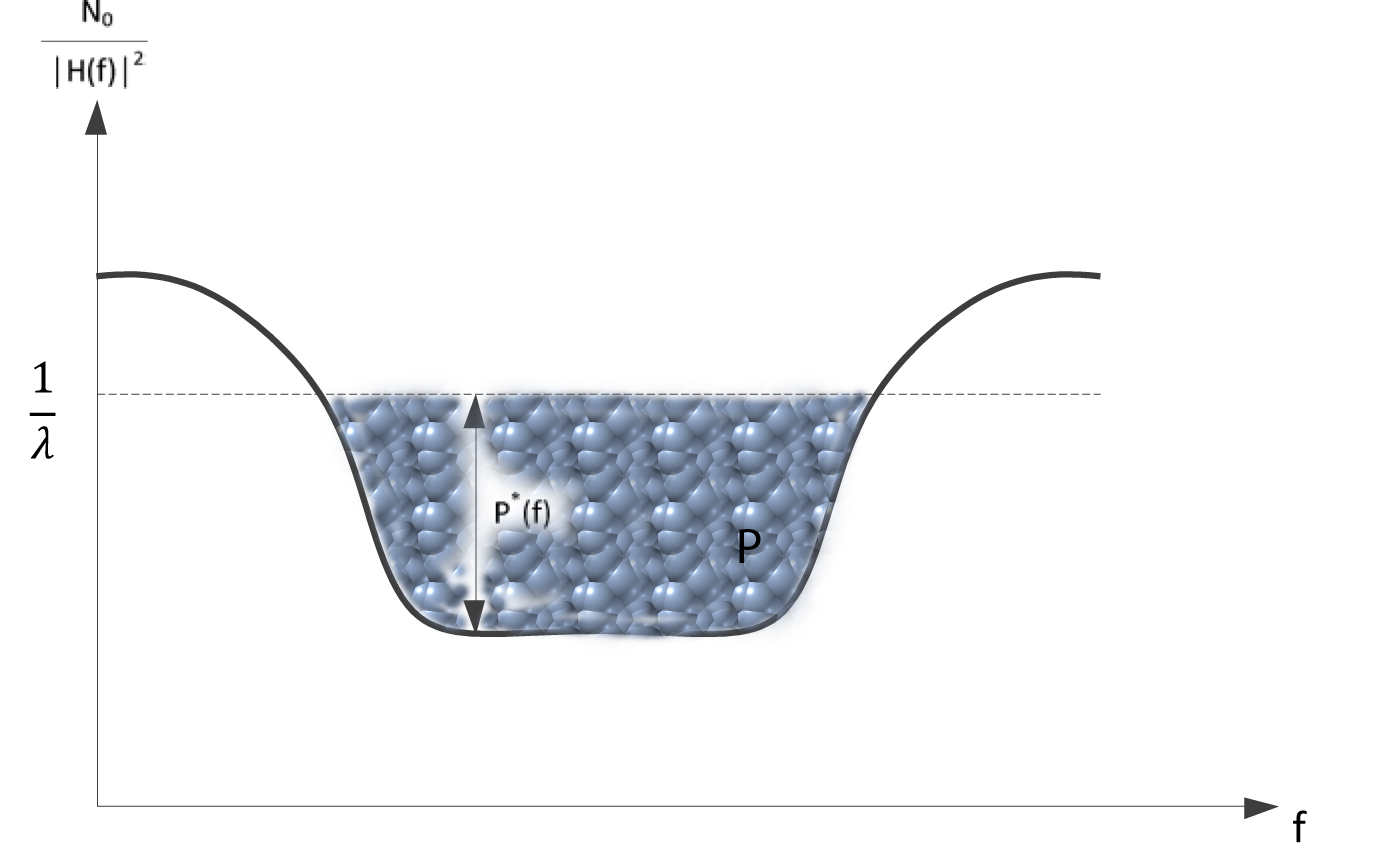
\includegraphics[width=6cm]{./bilder/Waterfilling.png}

\end{minipage}
